 \documentclass[10pt]{report}

\usepackage[frenchb]{babel}
\usepackage[T1]{fontenc}
\usepackage[utf8]{inputenc}
\usepackage{graphicx}
\usepackage{ccaption}

\graphicspath{{images/}}%dossier pour les images

\setlength{\hoffset}{-18pt}         
\setlength{\oddsidemargin}{0pt} % Marge gauche sur pages impaires
\setlength{\evensidemargin}{9pt} % Marge gauche sur pages paires
\setlength{\marginparwidth}{54pt} % Largeur de note dans la marge
\setlength{\textwidth}{481pt} % Largeur de la zone de texte (17cm)
\setlength{\voffset}{-18pt} % Bon pour DOS
\setlength{\marginparsep}{7pt} % Séparation de la marge
\setlength{\topmargin}{0pt} % Pas de marge en haut
\setlength{\headheight}{13pt} % Haut de page
\setlength{\headsep}{10pt} % Entre le haut de page et le texte
\setlength{\footskip}{27pt} % Bas de page + séparation
\setlength{\textheight}{708pt} % Hauteur de la zone de texte (25cm)

\title{Architecture des Applications Réparties\\ Rapport de Projet\\ Gestion d'un Tournoi de Football}
\author{Geoffrey CROCHET, Zo RABARIJAONA, Willy FRANÇOIS}
%\date{Vendredi 15 Novembre 2013}

\makeindex

\begin{document}

\maketitle


\newpage

\tableofcontents


\newpage
\chapter*{Introduction}

\chapter{Analyse UML}
\section{Diagramme de classes}
\subsection{Le modèle}
	\begin{figure}[here]
	      \begin{center}	      
		\fbox{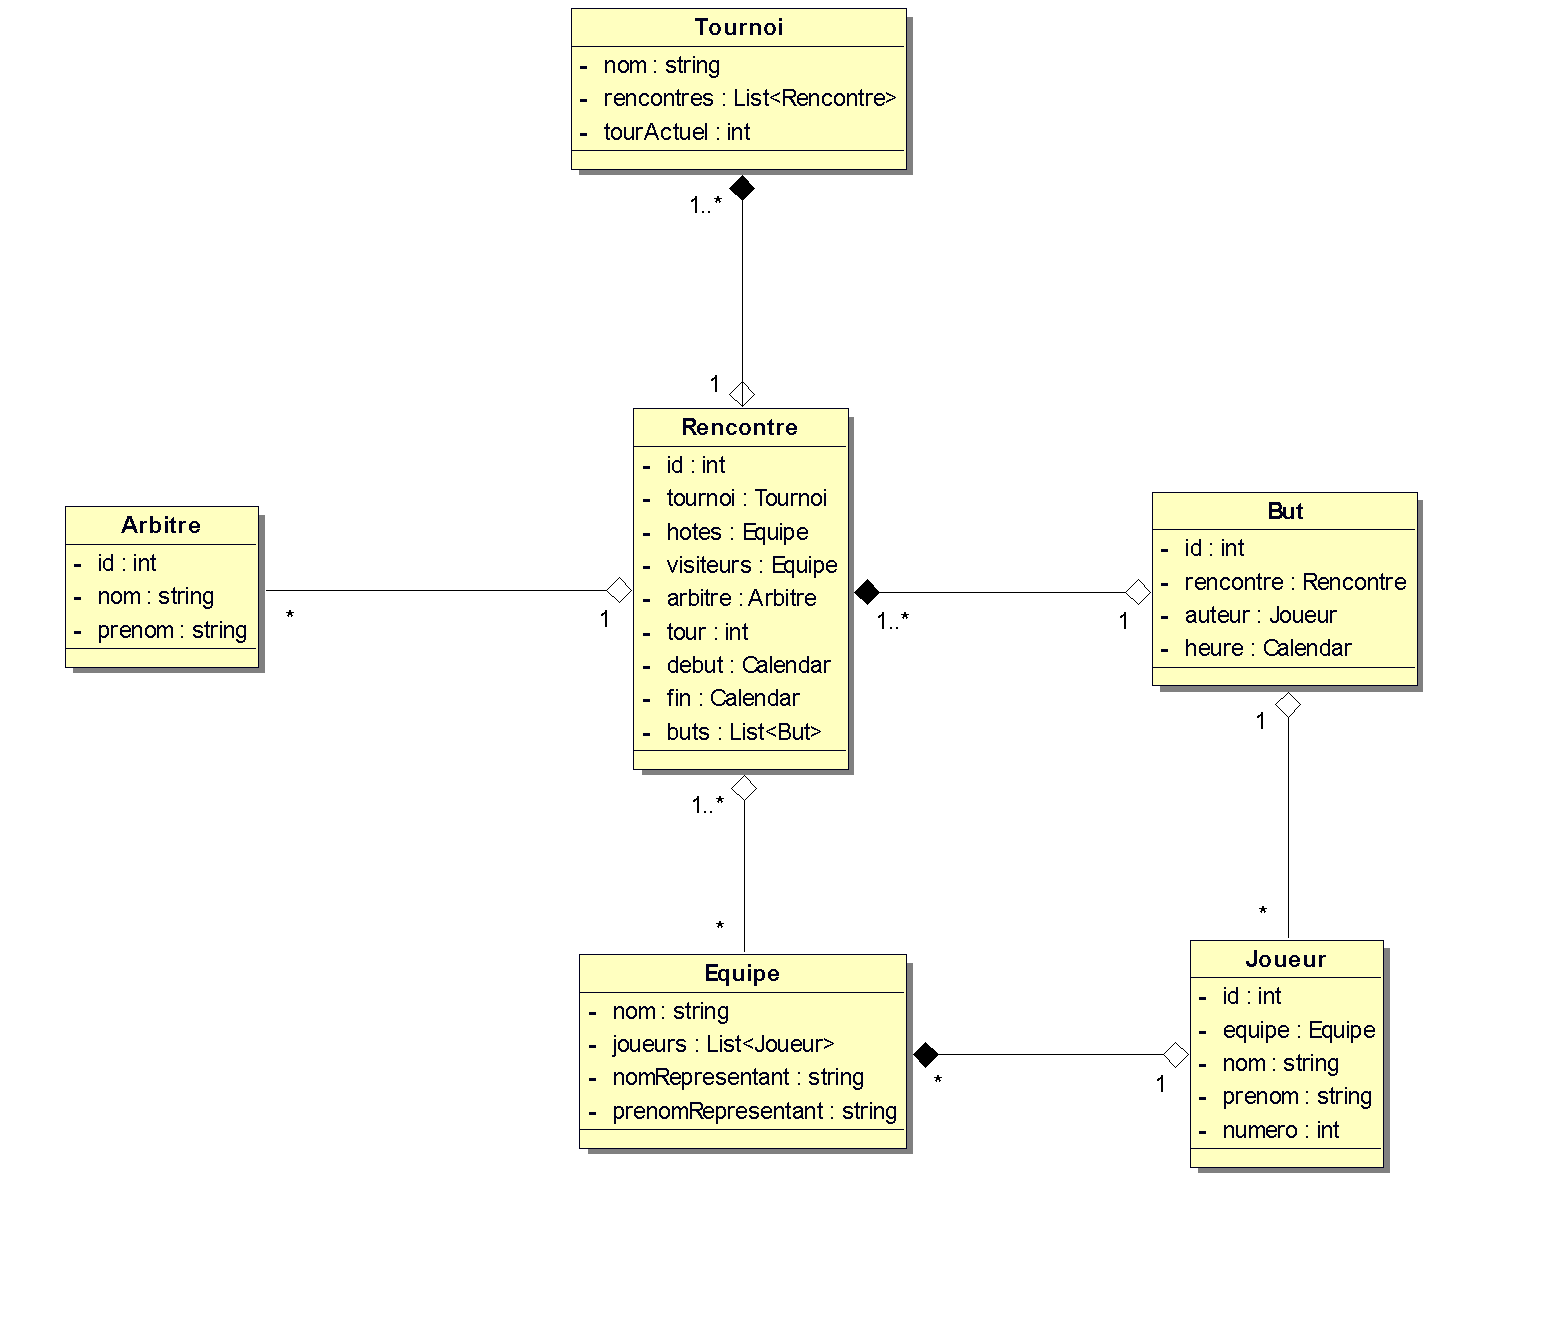
\includegraphics[scale=0.8]{class}}
	      \end{center}
	\legend{\underline{Diagramme de classes du modèle}}
	\end{figure}
~~\\
\subsection{Les Value Objects}

	\begin{figure}[here]
	      \begin{center}
		\fbox{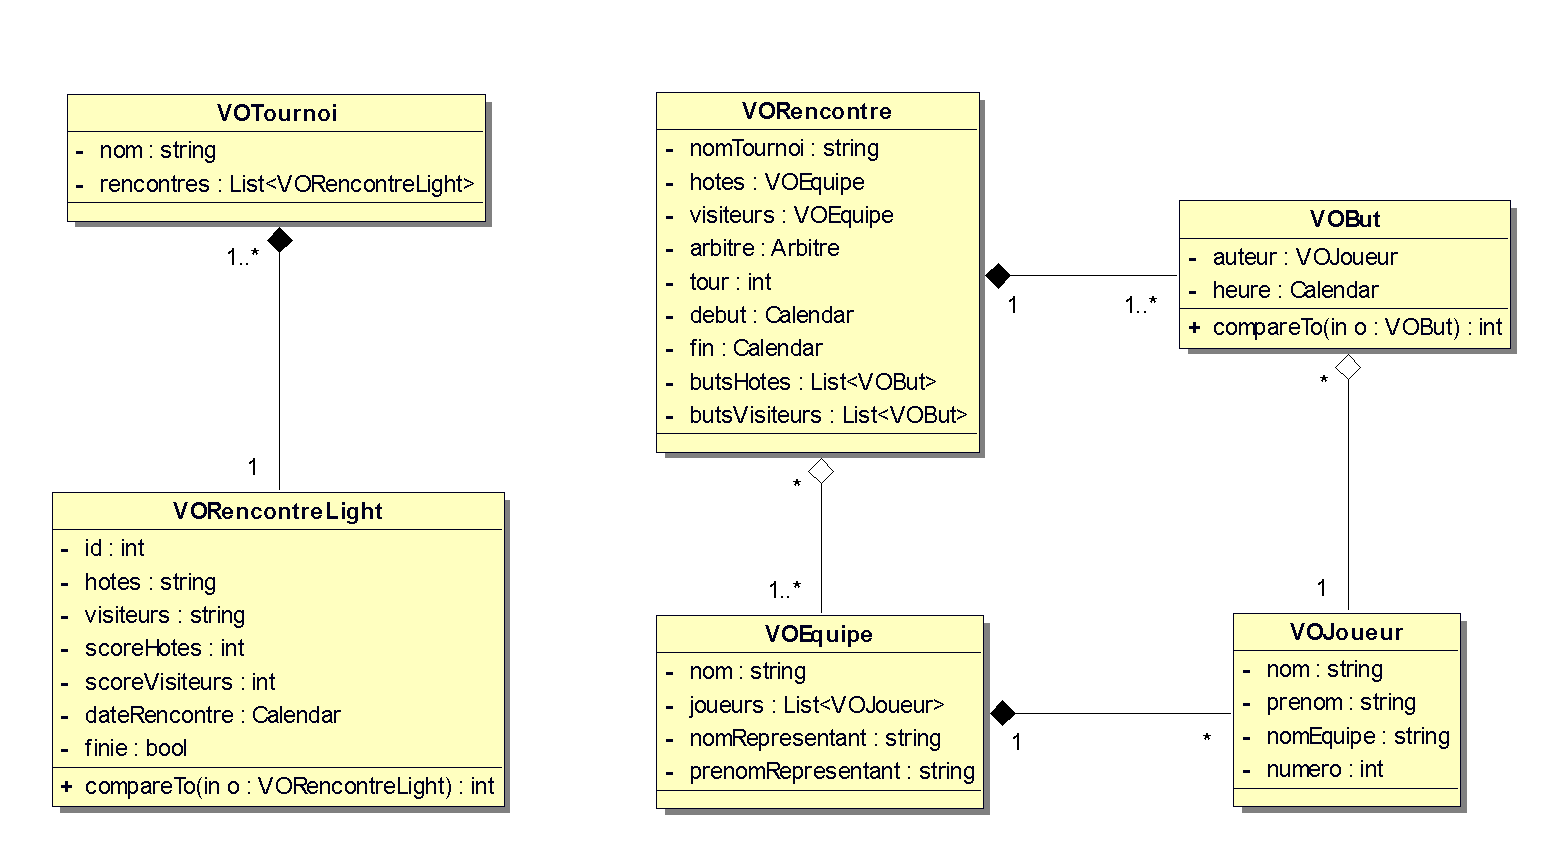
\includegraphics[scale=0.8]{vo}}
	      \end{center}
	\legend{\underline{Diagramme de classes des Value Objects}}
	\end{figure}
	
\subsection{Les EJB}
	\begin{figure}[hp]
	      \begin{center}
		\fbox{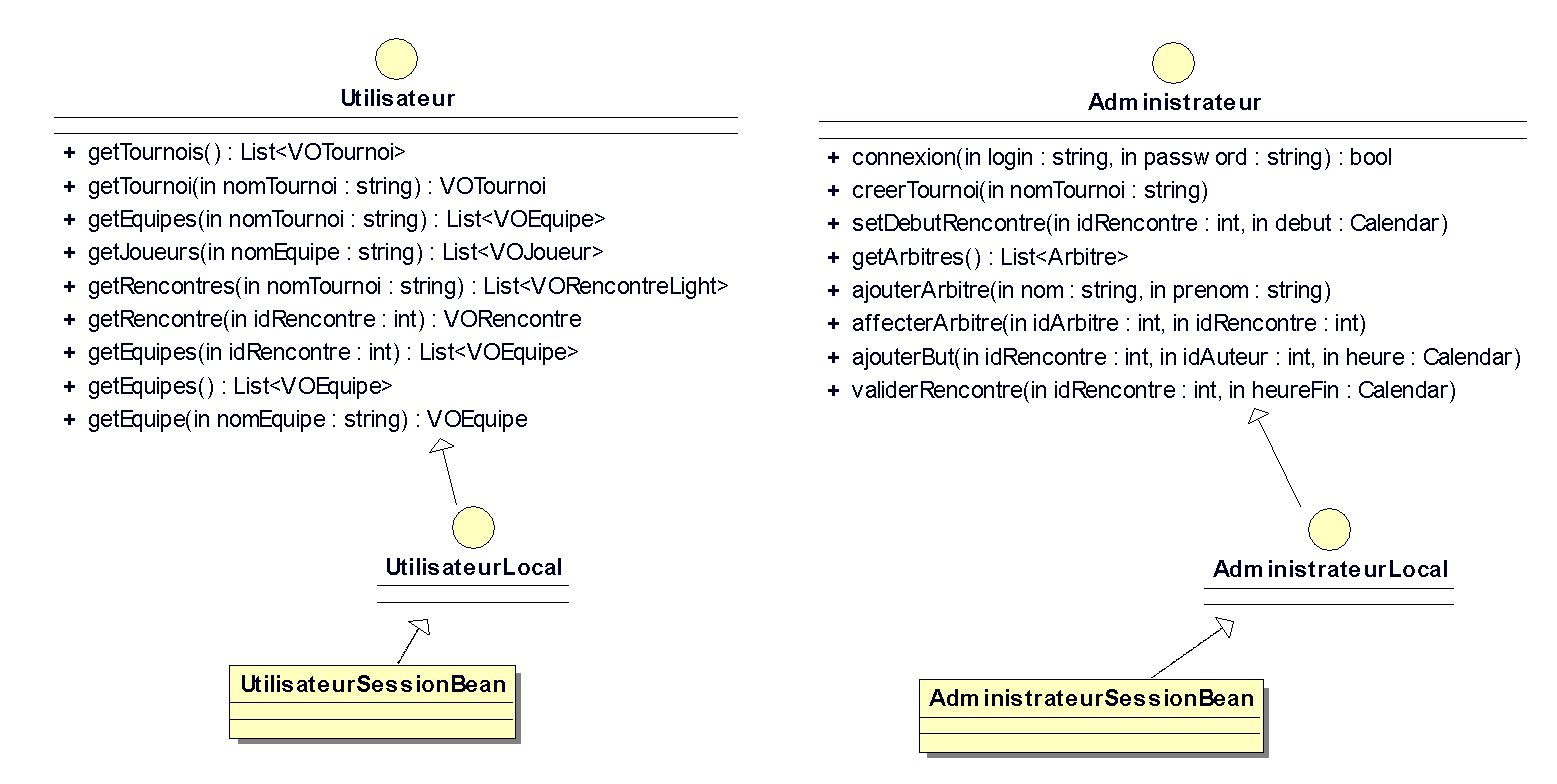
\includegraphics[scale=0.7]{ejb_ua}}
	      \end{center}
	\legend{\underline{Diagramme de classes des EJB Utilisateur et Administrateur}}	
	\end{figure}
	
	\begin{figure}[hp]
	      \begin{center}
		\fbox{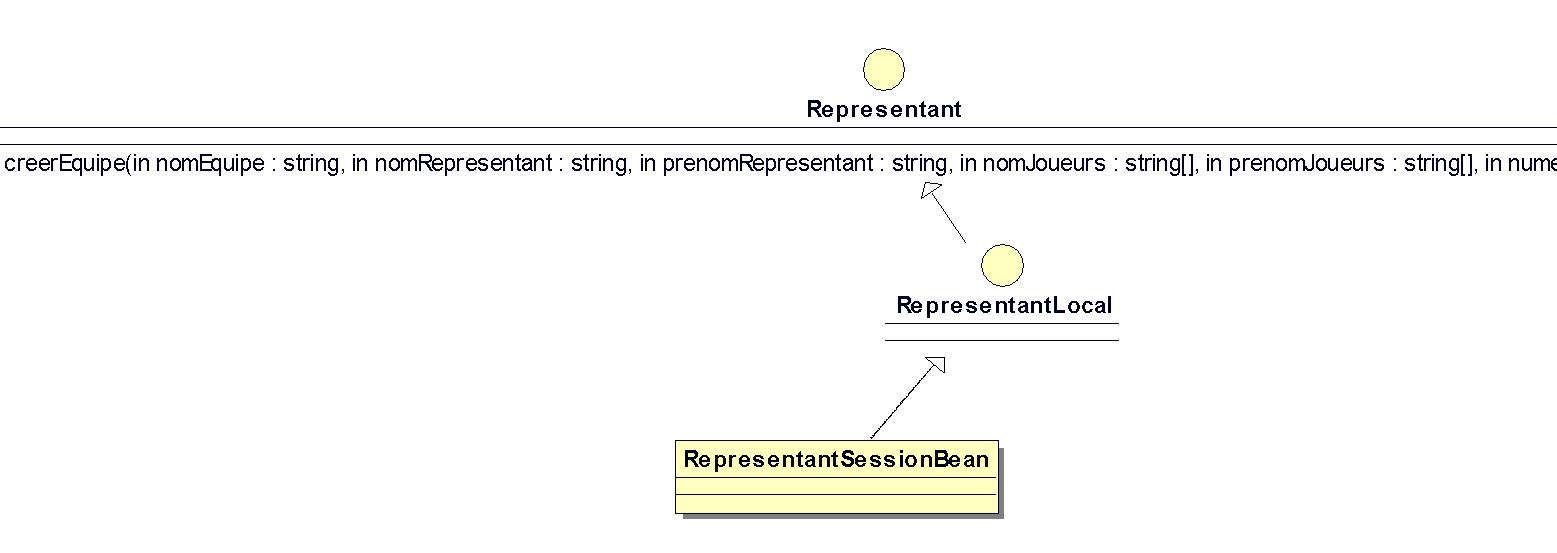
\includegraphics[scale=0.8]{ejb_r}}
	      \end{center}
	\legend{\underline{Diagramme de classes de l'EJB Représentant}}
	\end{figure}
	
	\begin{figure}[hp]
	      \begin{center}
		\fbox{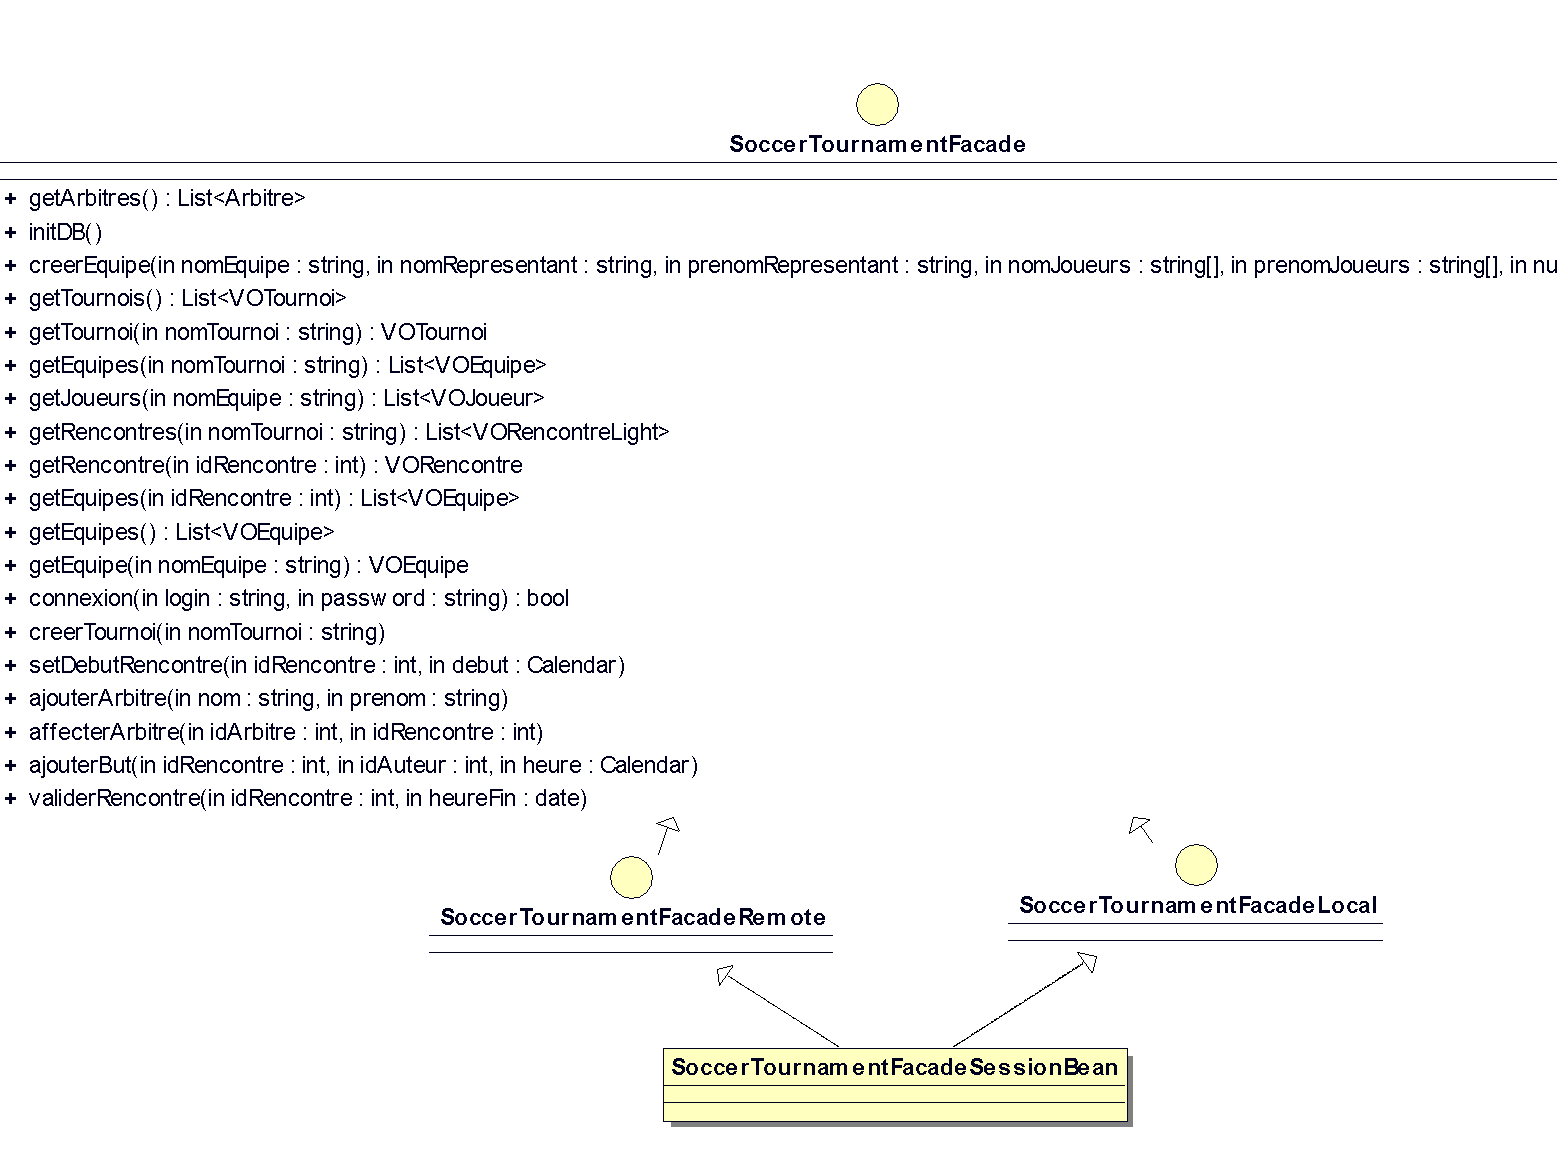
\includegraphics[scale=0.7]{ejb_session}}
	      \end{center}
	\legend{\underline{Diagramme de l'EJB Session façade}}
	\end{figure}	

\newpage
\section{Diagramme de cas d'utilisation}
	\begin{figure}[hp]
	      \begin{center}
		\fbox{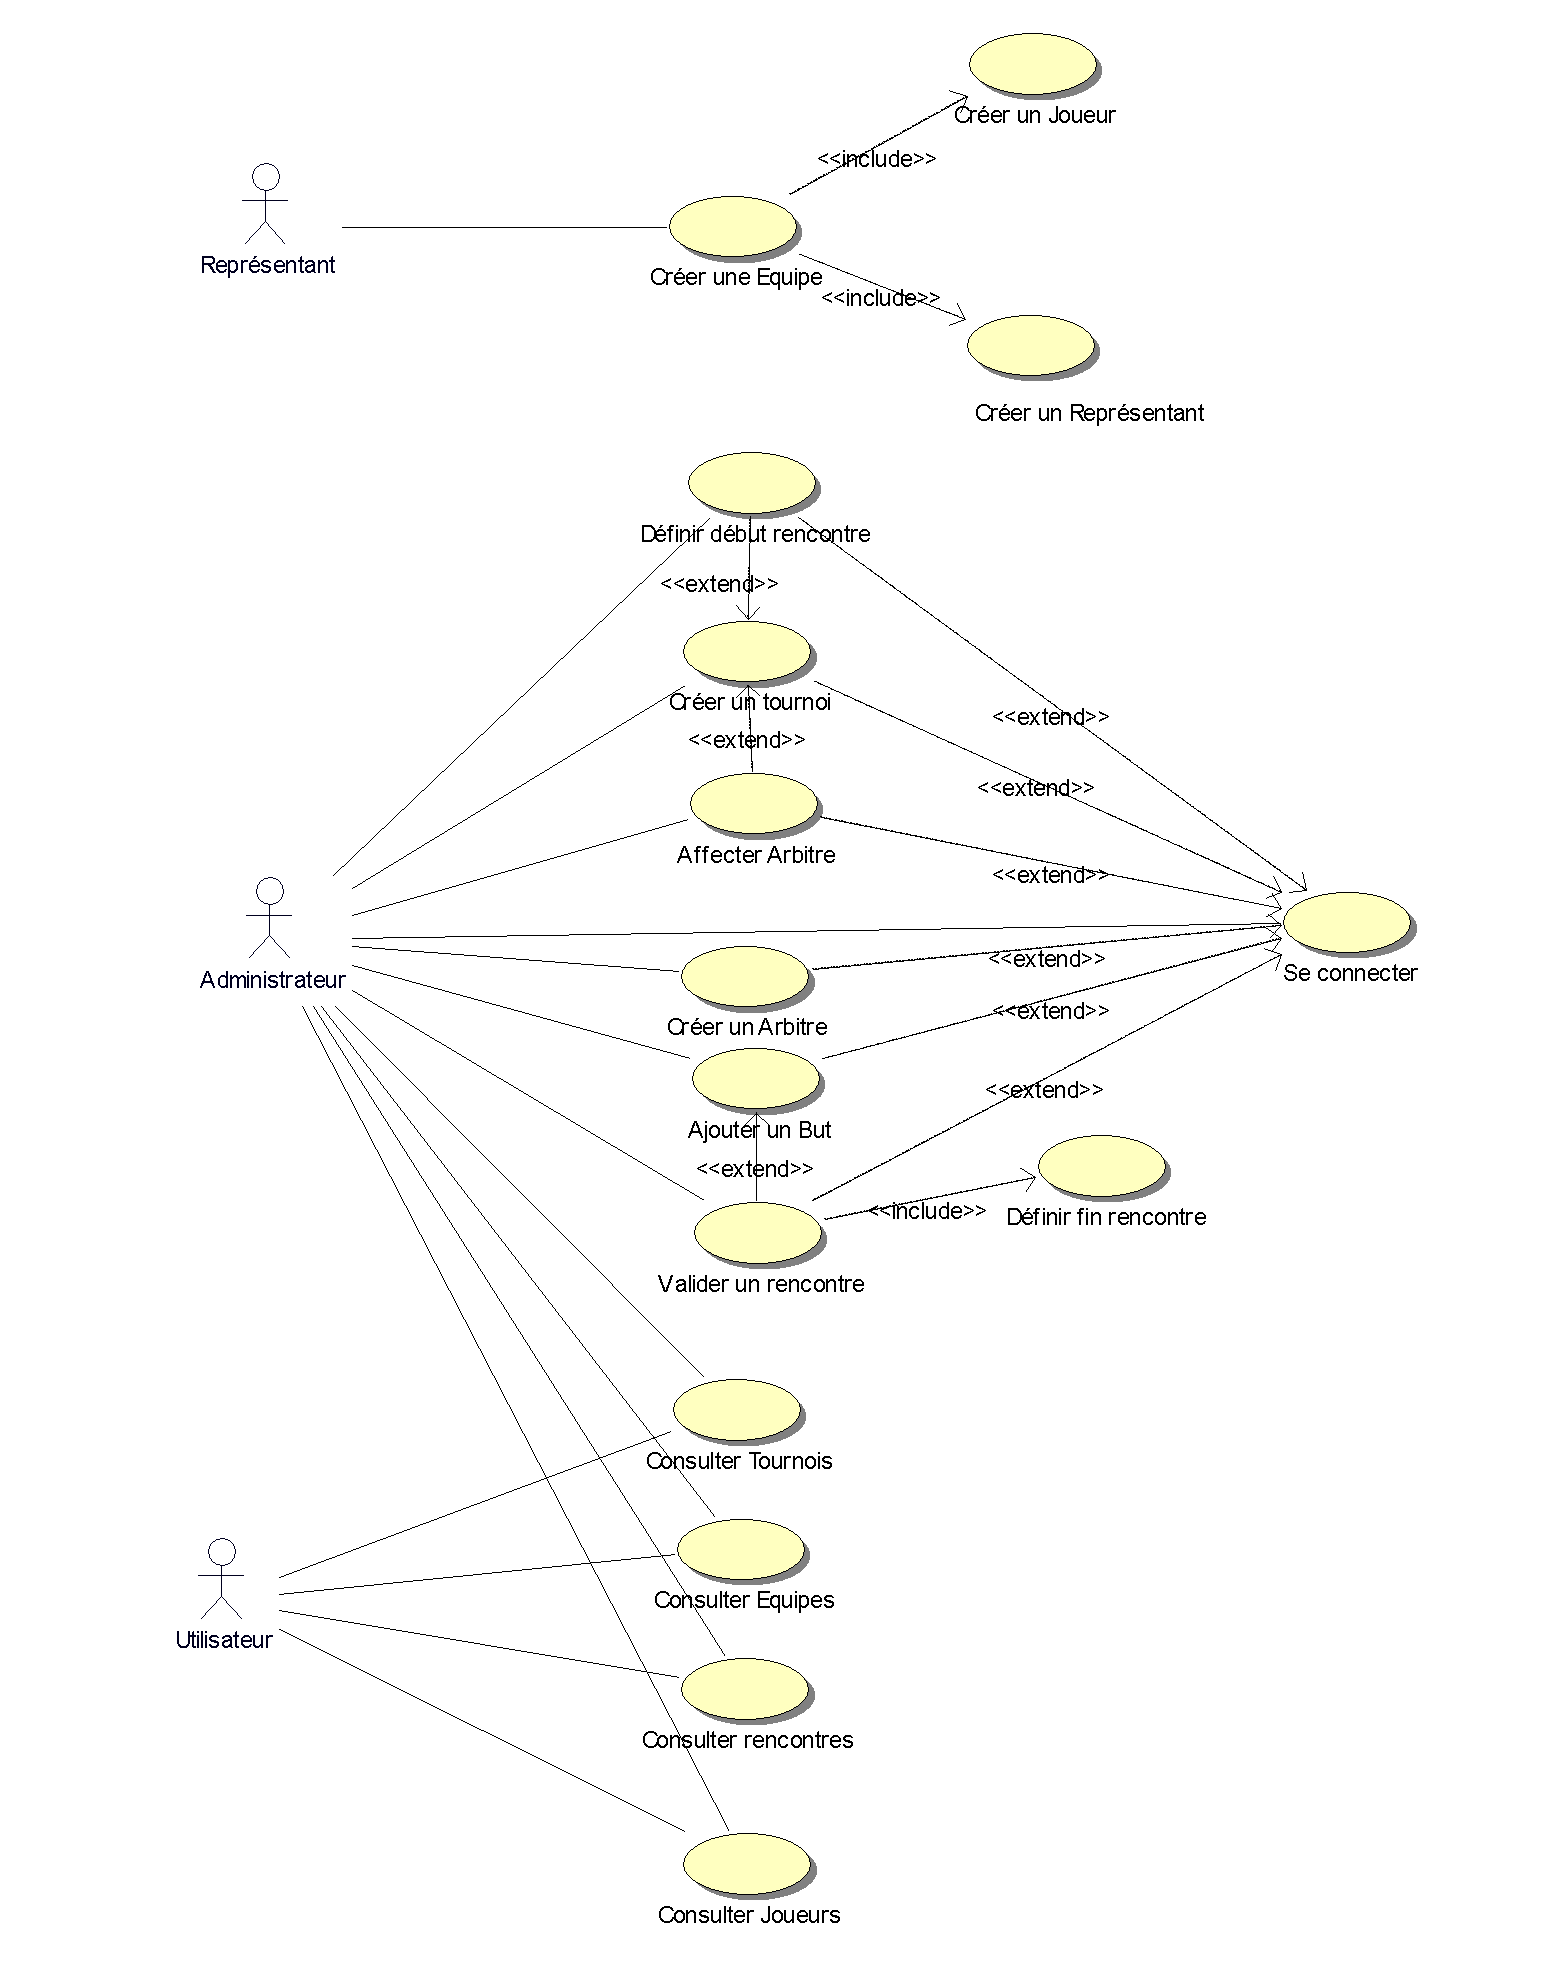
\includegraphics[scale=0.7]{use_cases}}
	      \end{center}
	\legend{\underline{Diagramme de cas d'utilisation}}
	\end{figure}

\newpage
\section{Schéma synthétique de l'application}
	\begin{figure}[hp]
	      \begin{center}
		\fbox{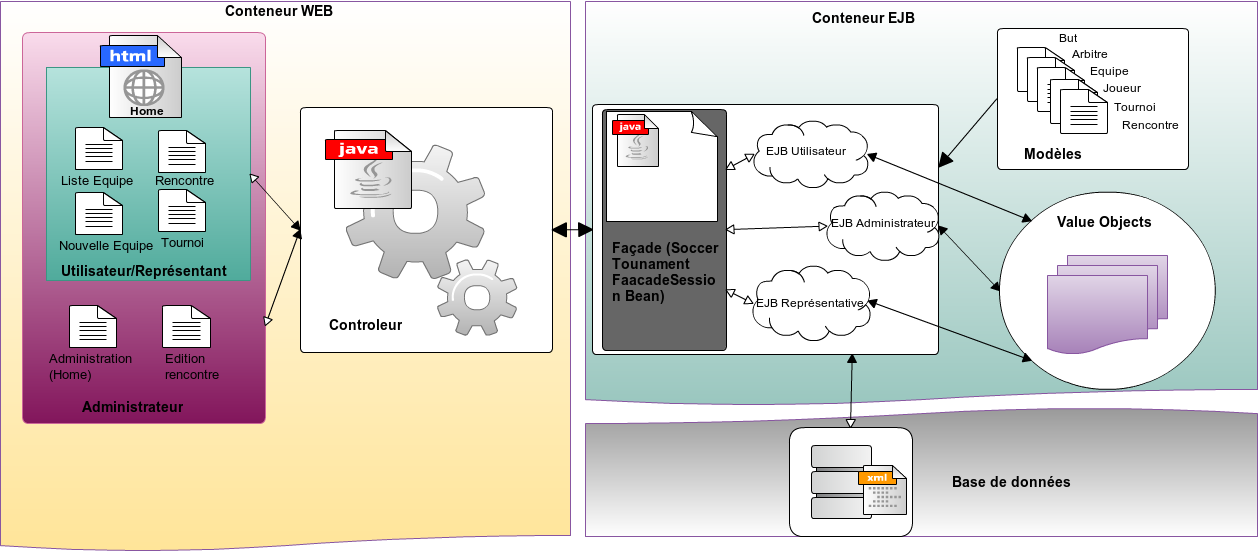
\includegraphics[width=18cm]{AAR}}
	      \end{center}
	\legend{\underline{Schéma synthétique de l'application}}
	\end{figure}

\newpage
\chapter{Répartition du travail}
\section{Gestion du temps de travail}
	\begin{figure}[hp]
	      \begin{center}
		\fbox{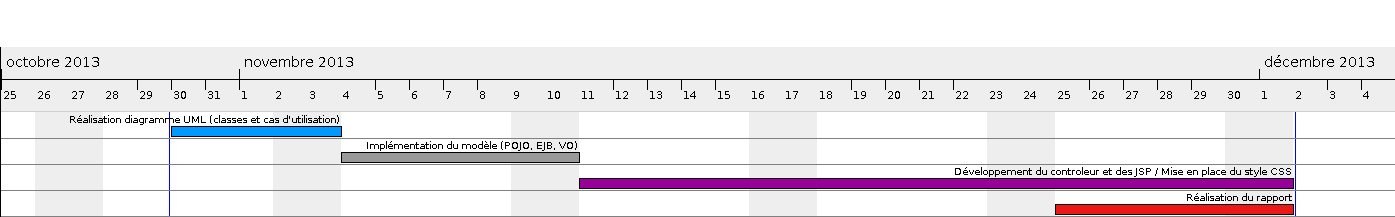
\includegraphics[width=18cm]{gantt}}
	      \end{center}
	\legend{\underline{Gestion du temps de travail}}
	\end{figure}
	
\section{Répartition des tâches}

\chapter{Guide d'utilisation}

\chapter*{Conclusion}

\end{document}
